\documentclass[t]{beamer}
\usetheme[deutsch]{KIT}
\setbeamercovered{transparent}
\setbeamertemplate{navigation symbols}{}

\KITfoot{}
\usepackage[utf8]{inputenc}
\usepackage{ngerman}
\usenavigationsymbols

\title{OQAT - Objective Quality Assessment Toolkit}
\subtitle{PSE - Abschlusspräsentation \\[0.3cm]
Alexander Monev $\cdot$ Artur Eckhart $\cdot$ Georg Emmantraut\\ $\cdot$ Johannes Sailer  $\cdot$ Sebastian
Leidig}

\institute[ITEC]{Institut für Technische Informatik}

\TitleImage[height=\titleimageht]{img/oqatLogo}

\AtBeginSection[]
{
  \begin{frame}
    \frametitle{Übersicht}
    \tableofcontents[currentsection]
  \end{frame}
}

\begin{document}

\begin{frame}
	\maketitle
\end{frame}

\begin{frame}
	\frametitle{Übersicht}
	\addcontentsline{toc}{section}{}
	\tableofcontents
\end{frame}

\section{Aufgabenstellung}
\begin{frame}
	\frametitle{Aufgabenstellung}
	\begin{center}
		\vspace*{\fill}
		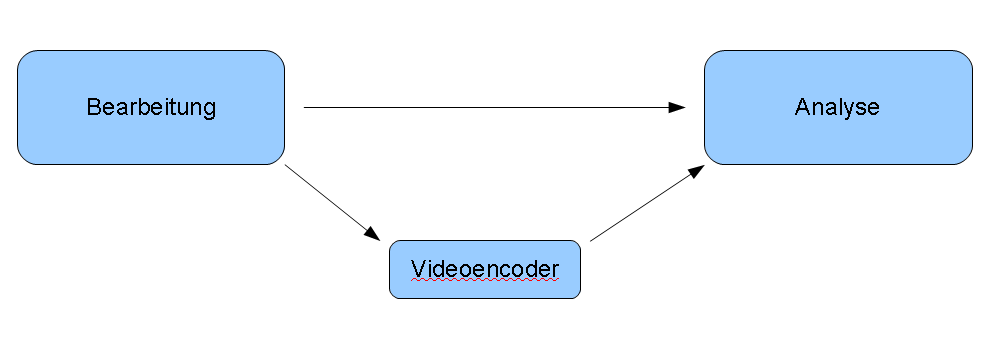
\includegraphics[scale=.35]{img/aufgabe.png}
		\vspace*{\fill} ~\\
	%	\onslide<2-> So kann man zeugs auf die ">nächste"< Folie packen. ~\\
	%	\onslide<3-> $ \Longrightarrow $ Würde man 5 hinschreiben wäre 
	%								dieser Punkt auch erst in 5 sichtbar
	\end{center}
\end{frame}
\section{Architektur}
\begin{frame}
	\frametitle{Noch ein Titel}
	% Die minipage umgebung teilt die Folie vertikal
	\begin{minipage}{5.5cm}
		
\includegraphics[scale=.29]{img/oqatLogo}	
	\end{minipage}
	\begin{minipage}{5.5cm}
		\begin{itemize}
		\item <+-> So läuft ne coole Aufzählung.
		\item <+-> Und hier ist dann die nächste
		\item <+-> Und noch eine.
		\end{itemize}
	\end{minipage}
\end{frame}
\section{benutzter Kram}
\begin{frame}
\frametitle{folientitel}
Inhalt
\end{frame}
\section{Statistiken}
\section{Vorführung}
\section{Fazit}
%	-entwurf simpler machen sollen
%	-auf johannes höhren
%	-Binding toll aber frisst zeit
%	-c#
%	-einarbeitungzeit> rest
%	-teamwork(blöd gut optimal?)
\end{document} 
